\documentclass{article}
\usepackage[utf8]{inputenc}
\usepackage{fullpage}
\usepackage[backend=biber,style=apa,backref=true]{biblatex}
\usepackage{listings}
\usepackage{xcolor}

\colorlet{punct}{red!60!black}
\definecolor{background}{HTML}{EEEEEE}
\definecolor{delim}{RGB}{20,105,176}
\colorlet{numb}{magenta!60!black}

\lstdefinelanguage{json}{
    basicstyle=\normalfont\ttfamily,
    numbers=left,
    numberstyle=\scriptsize,
    stepnumber=1,
    numbersep=8pt,
    showstringspaces=false,
    breaklines=true,
    frame=lines,
    backgroundcolor=\color{background},
    literate=
     *{0}{{{\color{numb}0}}}{1}
      {1}{{{\color{numb}1}}}{1}
      {2}{{{\color{numb}2}}}{1}
      {3}{{{\color{numb}3}}}{1}
      {4}{{{\color{numb}4}}}{1}
      {5}{{{\color{numb}5}}}{1}
      {6}{{{\color{numb}6}}}{1}
      {7}{{{\color{numb}7}}}{1}
      {8}{{{\color{numb}8}}}{1}
      {9}{{{\color{numb}9}}}{1}
      {:}{{{\color{punct}{:}}}}{1}
      {,}{{{\color{punct}{,}}}}{1}
      {\{}{{{\color{delim}{\{}}}}{1}
      {\}}{{{\color{delim}{\}}}}}{1}
      {[}{{{\color{delim}{[}}}}{1}
      {]}{{{\color{delim}{]}}}}{1},
}


\usepackage{url}
\usepackage{graphicx}
\graphicspath{./figs}
\usepackage{amsmath}
\usepackage{hyperref}
\hypersetup{colorlinks=true, citecolor=blue}

%for including wordcount in file
\immediate\write18{texcount -template="{word} words in main body, excluding headers and bibliography." \jobname.tex -out=\jobname.sum}
\usepackage{verbatim}
\usepackage{setspace}
\doublespacing
\newcommand\wordcount{\verbatiminput{\jobname.sum}}


\author{George Tyler}
\date{\today}

\addbibresource{diss.bib}
\begin{document}

\title{Social Media, Risk Perception, and Social Distancing: \\ Evidence from 15.3 Million Geolocated Tweets}

\maketitle

\abstract{Does social media predict risk-taking behaviour? I investigate this question in the context of COVID-19 by exploiting a large panel of tweets. Using inferred and explicit geolocation data embedded in the tweets, I study the extent to which public expressions of sentiment influence social distancing, as measured by GPS-located smartphone data.}
\wordcount

\tableofcontents

\section{Introduction}
\subsection{Overview}
The early stages of the COVID-19 pandemic saw an unprecedented shift in behaviour for most citizens of the United States. In a short period of time, a large number changed their habits of working, socialising, and travelling. They did so both as a result of government restrictions in the form of non-pharmaceutical interventions (NPIs) and as a private response to the spread of the pandemic. Economists have taken interest in how citizens formed these behaviour changes, and the role that beliefs and risk attitudes played in determining the response to public policy. A new way to measure belief formation and public sentiment is with social media, an increasingly common platform for expression of opinion. It is plausible that those who express more risk-averse sentiment towards COVID online will be inclined to respond in a stricter fashion to social distancing and other public health regulations. In this dissertation, I study the impact of local expressions of risk attitude on public behaviour in the early months of the pandemic. Specifically, I study whether a measure of risk-averse sentiment on Twitter is linked to increased social distancing behaviour at the county/week level. 

This dissertation contributes to two strands of the recent economics literature on the COVID-19 pandemic. First, it investigates the relationship between partisanship and risk preference. Previous papers posit that political preference influences social distancing through risk preference; I contend that \textit{local} risk preference is a separate factor to political partisanship, and has an independent impact on social distancing. More broadly, the paper investigates the relationship between risk preference and economic behaviour, and presents a novel example of economic inference from social media using text analysis. 


A key vector for expressing sentiment is social media, with Twitter and Facebook's suite of products\footnote{Facebook, Facebook Messenger, Instagram, and WhatsApp} being the most widely-adopted, each platform having over 80 million monthly active users in the US. A survey by the Pew Research Foundation indicates that 22\% of US adults use Twitter, with 42\% of these using it on a daily basis \parencite{perrinShareAdultsUsing2019}. On Twitter, users can share their own text, with the option to link to a website; alternatively, they can `retweet' another user's text or link. Users can also use `hashtags' in their tweet, which connects their tweet to a particular topic. If the user has allowed it, Twitter also records the location of the tweet; and it is also possible for the user to set their location on their profile. In this way, it is possible to create a panel of geographically-located tweets about a particular topic. 

I exploit GeoCov19 \parencite{qaziGeoCoV19DatasetHundreds2020a}, a dataset of 524 million geolocated tweets, to measure the local public sentiment on COVID in the US. The tweets cover the period from 1st February to 1st May, the period I focus on. The particular subset of the data I use contains 33.36 million tweets in total; a small subset are exactly geolocated (the user has provided a GPS location), while most are inferred from the location tab in the user's profile. The tweets were collected using the Twitter Streaming API, querying for tweets containing any of a list of 800 COVID-related keywords. I also use anonymous smartphone location data, collected by the company SafeGraph, as a measure of the extent of social distancing in an area. I present two measures of social distancing at county level: first, the median minutes spent at home during 8am-6pm; second, the proportion of measured devices that stayed at home all day \parencite{safegraphinc.SocialDistancingMetrics2020}. Demographic controls are also acquired and presented from the American Community Survey and the 2010 US census. 

I use dictionary-based text analysis to assess the level of risk sentiment in a tweet. More sophisticated methods of text analysis like latent factor modelling are discussed in the Methods section. In the absence of a lexicon of risk preference, the NRC Emotion Lexicon \parencite{mohammadCrowdsourcingWordEmotion2013} is used. This is a widely-used mapping of English words to eight basic emotions (anger, fear, anticipation, trust, surprise, sadness, joy, and disgust). Starting from a set of tweets that mention COVID, I assign tweets containing fear-associated words to a risk-averse sentiment. The base unit of analysis is the county-week; as such, I measure the proportion of tweets that contain fearful language in each county and week. 

It is plausible that social media is a valid measure for risk appetite. The intuition is that the textual content of a social media post broadly reflects the poster's current opinion of a topic: for example, in response to the first confirmed US COVID death on February 26th, a user might express fearful sentiment, or a neutral sentiment. This opinion of the topic, particularly their level of fear, maps to a user's broader expectations about the course of the pandemic: while other emotions like joy, anticipation, and trust may rely on the context of the discussion, expressions of fear are plausibly consistent in mapping to risk-averse sentiment. When restrictions are implemented, users who initially formed pessimistic expectations may be more inclined to adhere more to them than a user who formed optimistic or netural expectations. The key aspect to the data is that the Twitter conversations provide a real-time insight into local sentiment as NPIs are implemented; this sentiment changes both in response to current, local experience \textit{and} broader partisan interpretations of current events.

The primary econometric specification is a panel model with county and week fixed effects;
\[Y_{it} = \alpha + \beta r_{it} + \mu c_{it} + \tau_i + \delta_t +  X_{it}\gamma + \epsilon_{it}\]
where \(Y_{it}\) is a vector of social distancing metrics, \(\beta r_{it}\) is the risk perception measure, (i.e. the proportion of total tweets containing fearful language), \(\mu c_{it}\) the number of COVID cases, \(\tau_i + \delta_t\) county and week-level fixed effects, and \(X_{it}\gamma\) demographic controls.


This research contributes to the recent economics literature seeking to explain the disparities in social distancing in the early stages of the pandemic in the US. In particular, partisanship has been shown to be a significant factor on the practice of social distancing: \textcite{allcottPolarizationPublicHealth2020,barriosRiskPerceptionLens2020,painterPoliticalBeliefsAffect2020} show that areas with more Republicans engaged in less social distancing, are associated with lower perceptions of risk of the pandemic, and exhibited less remote transactions. \textcite{simonovPersuasiveEffectFox2020,ananyevSafestTimeFly2020} also measure the causal effect of the right-wing Fox News network on social distancing during the pandemic. This paper builds on \textcite{barriosRiskPerceptionLens2020} in particular, which shows that online risk perception is predicted by Trump voter share: by measuring risk perception with a high-frequency geolocated dataset, my approach controls for political alignment and assesses the effect of risk perceptions on their own. In essence, I measure expressions of sentiment regarding COVID risk, and given this data I ask whether local risk sentiment predicts social distancing behaviour beyond political affilitation. Second, this research relates to the recent economics literature around heterogeneous-agent epidemiological models, which endogenise individual behaviour -- including social distancing -- into the effective reproductive number \(R(t)\). These recent models, such as \textcite{acemogluTestingVoluntarySocial2020,brotherhoodEconomicModelCOVID192020,eichenbaumMacroeconomicsEpidemics2020}, assume that preferences over risk are predictive of social distancing behaviour; this paper looks to empirically confirm this key assumption.

%This paper is particularly close to two research papers, This dissertation takes a similar approach, but uses Twitter as a news source instead. More broadly, this dissertation contributes to the literature on the effects of misinformation and political affiliation on public behaviour.

This dissertation also contributes to the rapidly-expanding field of text analysis in economics, and presents an example of how the rich sentiment data encoded in social media communication can inform insights into public behaviour. This topic is particularly mature in finance -- where sentiment data from public company documents, news media, and social media have been shown to predict stock market reactions \parencite{bollenTwitterMoodPredicts2011} -- and monetary economics, where central bank statements, coded according to their attitude to inflation, predict fluctuations in Treasury securities \parencite{luccaMeasuringCentralBank2009,gentzkowTextData2019}. On the topic of empirical economics, this paper takes a similar approach -- by using online data to predict local sentiment -- as \textcite{stephens-davidowitzCostRacialAnimus2014}, which uses Google search data to proxy an area's racial animus, and uses this to estimate the Obama vote share. I use geolocated Twitter sentiment to proxy the local attitude to COVID in a given week, and test to see if this predicts social distancing practice. 

The argument of the dissertation rests on the following assumptions: first, that social media data is a valid proxy for local risk appetite, and that fear-associated language in COVID-related tweets is an effective estimator of the risk appetite encoded in the tweet. It is also important to note a possible selection effect in the dataset: tweets about COVID may attract a greater level of fear-related language and not reflect an individual's true opinion about social distancing and other preventative measures. I address these assumptions and drawbacks and discuss methods to alleviate them in the Results section.


\section{Literature Review}%Aim: 3000 words
\subsection{Text analysis and sentiment mining in Economics}
\textit{Context and applications of Text Analysis in economics; technical section describing the various methods used in the literature is in the methods section.}
\subsection{Usage of `Digital Trace' and geolocation datasets in economics}
\textit{General; description of previous uses of geolocation data}
\subsection{COVID-19: Empirical estimates of drivers of social distancing behaviour}
\textit{Summary of empirical research on COVID}
\subsection{COVID-19: Models of risk perception and social distancing}
\textit{Discussion of different augmentations to SIR models; incorporation of endogenised social distancing / individual choice. Particular focus on risk-attitude heterogeneity.}
At the outbreak of the pandemic, many economists augmented the standard epidemiological `Susceptible-Infected-Recovered' (SIR) models with economics-derived models of human behaviour. \textcite{murrayEpidemiologyTimeNeed2020}, writing as an epidemiologist, identifies 
\subsubsection{Standard SIR model}
\textcite{kermackContributionMathematicalTheory1927} introduced the SIR model and it remains the basis for most modern epidemiological models; this explanation follows \textcite{averyEconomistGuideEpidemiology2020}. Each member of the population can be in one of three `Susceptible, Infected, Recovered' states; therefore, at each time period we have

\begin{equation}\label{SIRstates}
    S(t) + I(t) + R(t) = 1
\end{equation}
, where the population is normalized to 1. A susceptible individual can only move to the infected state through contact with an infected individual, and an infected individual can only move to the recovered state. The recovered state, in the base version, includes \textit{both} those who have recovered and those who have died: they share the key characteristics of being noninfectious and not susceptible to future infection. Three key parameters govern the rate of transitions between these states: \(\gamma\), the recovery rate, represents the probability per unit time for an individual to move from Infected to Recovered; \(R_0\), the basic reproductive number, is the ``number of people an infectious person would infect over the course of their disease in a fully susceptible population'' \parencite[81]{averyEconomistGuideEpidemiology2020}. \(R_0\) therefore stands in an inverse relationship with the recovery rate: \(R_0 = \beta / \gamma\), where \(\beta\) is the expected number of contacts an individual makes per unit time in normal circumstances. Assuming that the individual infects every contact, the states evolve according to 

\begin{align}
    \dot{S}(t)&= -S(t)I(t)R_0 \gamma \\
    \dot{I}(t)&= S(t)I(t)R_0 \gamma - \gamma I(t) \\
    \dot{R}(t)&= \gamma I(t)
\end{align}
. For epidemiologists, then, \(R_0\) is seen as a `compound parameter' of both the virus' natural infectivity\footnote{Which itself is governed by the expected length of contagiousness \(\frac{1}{\gamma}\) and the transmissibility, which we assume to be 1.} and the expected number of in-person interactions during pre-pandemic life \parencite[84]{averyEconomistGuideEpidemiology2020}: government policies and behaviour change therefore have the effect of reducing the \(R_0\) parameter to some variable \(R^t_0\). This gives rise to the key aim of `flattening the curve': achieving a state where -- given the current susceptible fraction of the population -- the expected number of people that a contagious individual infects over the course of their illness is below 1:
\begin{equation}
    R_t \equiv R^t_0 S(t) < 1
\end{equation}. \(R_t\) is known as the effective reproductive number.

\textcite{averyEconomistGuideEpidemiology2020} sorts the contributions of economic research to the basic SIR model into three basic categories: pointing out the endogeneity of the reproductive number, adapting the model to heterogeneity of different subpopulations, and adapting SIR models to policy-relevant issues like social distancing compliance. I now set out the insights that model-based COVID economic research gives to the topic in this dissertation: the relationship between risk preferences, local demographic characteristics, and social distancing behaviour.


\subsubsection{Models of endogenous social distancing}
In the base SIR model, \(R^t_0\) is endogenous, since individuals adjust their exposure to others in response to the state of the epidemic. A priority for this dissertation is to establish the characteristics and determinants of social distancing; a large body of literature has emerged in economics discussing this issue. 

\textcite{toxvaerdEquilibriumSocialDistancing2020} models individuals as making non-cooperative, forward-looking decisions to engage in costly social distancing by solving a tradeoff against beneficial social behaviour and the risk of infection. Toxvaerd finds that equilibrium social distancing depends on the threshold infection probability, which is determined by the aggregate disease prevalence; this entails that individuals react to higher prevalence by distancing more, mitigating the flow rate between \(S(t)\) and \(I(t)\). In this model, individuals assess the value of becoming infected as equal to the expected discounted lifetime utility of being in the infected state. The model considers a homogenous population and so does not take demographics into account.

\textcite{farboodiInternalExternalEffects2020} also models the tradeoff of exposure against health risks. Using the SafeGraph dataset, they find that social activity levels fall before imposition of mandatory measures. This yields their key observation: desire to avoid illness is a key determinant of social distancing, meaning that there is a strong laissez-faire reduction in social activity. This cost-response reduction produces the majority of social distancing behaviour, but not enough for optimal pathogen suppression; as such, social distancing orders are recommended. They implement quadratic matching with random search, introduced in \textcite{diamondEquilibriumAnalysisSearch1979}, to model social interactions. Individuals are split into the S, I, R states, where the level of chosen social activity is the same among all individuals in that state. Disease transmission is therefore a function of \(\beta\), the number in the susceptible and infectious states, and the social activity level of each of those states. Individuals choose their level of social activity, taking the external social activity level and the number of infected as a given. The model, however, abstracts from subpopulation heterogeneity.

\textcite{eichenbaumMacroeconomicsEpidemics2020} also point out that exposure comes either from purchasing consumption goods, from working, and from random interactions such as touching surfaces: this shows the importance of income and mode of work for disease transmission. 

\textcite{goolsbeeFearLockdownDiversion2021} 
\subsubsection{Subpopulation heterogeneity}

\subsubsection{Endogenous social distancing and policy models}

\section{Text analysis: an overview}\label{textan}
In the literature review I summarised the current uses of Text Analysis in the economic literature. In this section, I present a detailed look at the inference problem for text analysis of English documents, and the various types of approaches possible to tackle it. The section introduces concepts that are used in the later Methods section, and also serves as an introduction to the field of text analysis for economics.
\subsection{The inference problem}
For economists, the fundamental concept is that relevant information exists within a corpus of text. This information can be represented as a low-dimensional variable, relevant to a model of economic decisionmaking: for example, interest rate expectations or risk aversion. However, this low-dimensional variable is expressed in text, a noisy, extremely high-dimensional format: a list of documents which are \(n\) words long, drawn from a vocabulary of size \(p\), has a dimension of \(p^n\). Given this computational constraint, the central challenge is to isolate the latent variable from the high-dimensional noise in a robust manner.  \textcite{gentzkowTextData2019} present a useful notation for a two-step process of this extraction: first, the raw text \(\mathcal{D}\) is mapped to an array of tokens, \(\mathbf{C}\). These tokens -- usually in the form of words, phrases, or sentences -- are the fundamental units of analysis. Second, the token array is mapped to the outcome array \(\hat{\mathbf{V}}\), which is an estimate of the latent variable \(\mathbf{V}\). \(\hat{\mathbf{V}} \) is then used in the final analysis. In these two mappings, there are two challenges: first, to include only tokens relevant to the variable in \(\mathbf{C}\); second, to accurately estimate  \(\mathbf{V} \) using \(\mathbf{C}\). 

\subsection{Mapping \(\mathcal{D}\) to \(\mathbf{C}\): text pre-processing}
In \textcite{gentzkowTextData2019}'s notation, the vector \(\mathcal{D}\) is the corpus of text to be analysed, consisting of documents \(\mathcal{D}_i)\): a central bank announcement, for example. \(\mathbf{C}\) is a numerical matrix, where the columns correspond to tokens, and rows correspond to documents.\footnote{It is sometimes called the `Document Term Matrix (DTM)'} \(\mathbf{C}_{ij}\) is a scalar representing the \textit{term frequency}: how many times each token appears in a document. In other words, \(\mathbf{C}\) is a frequency matrix, with each member of the matrix representing the counts in a document of a particular token. Each column is an element of the vocabulary -- the set of unique tokens in the whole corpus -- and so the number of columns equals the size of the vocabulary. Representing raw text in this fashion is a central part of the \textit{information extraction} problem \parencite[529]{manningFoundationsStatisticalNatural1999}. Ultimately, we wish to discard all tokens which do not convey information relevant to the latent variable, and quantify the amount of information each token conveys.

The first decision is to define the token. The simplest method is to assign tokens to single words, or `unigrams'. This method, known as the `bag-of-words', reduces the dimensionality of the document by the maximum amount by ignoring any dependence between the tokens. However, it simplifies language to a large extent, as (by definition) word order, grammar, ambiguous terms (``hard'', ``line''), and modifiers (``not'') are lost in the mapping. These problems can be moderated by instead considering \(n\) consecutive words to be a token: ``in the beginning'' maps to (``in.the'', ``the.beginning''. Since the words overlap, the size of \(\mathbf{C}\) increases exponentially, requiring a corresponding increase in computational power. \(\mathbf{C}\) also becomes more sparse, requiring more observations. However, even considering pairs of words yields a significant improvement in extracting meaning \parencite{chengNgramSkipgramConcgram2006}, as we expand the remit to two-word phrases. As computational power has increased, it is possible to efficiently include a wider context than 2- or 3-grams by using the word embeddings technique.

There are several steps that can reduce the size of the vocabulary -- the number of columns of \(\mathbf{C}\) -- without a great degree of information loss. When the bag of words method is used, \(\mathbf{C}\) is a word frequency matrix. It will therefore reflect the structure of English in that each document will have a large frequency of structural words like ``from'', ``the'', ``could''. These are called stop-words, and do not convey meaning; the first step of a text analysis is to remove these words by filtering on a list. There are standard lists, but it is important to take the domain of the corpus into account when filtering stop-words; for example, Twitter has domain-specific stop-words ``@'', ``\#'', but filtering punctuation risks removing emoticons (``:)''). A closely related step is converting all words to lowercase, on the general assumption that word meaning does not depend on whether it starts a sentence \parencite{dennyTextPreprocessingUnsupervised2018}. However, in the context of social media, this may be problematic: emotion and intensity of sentiment is often expressed by various forms of capitalisation. Internet-targeted sentiment analysers usually attempt to take this into account. Words are also expressed in English in different forms (``laughing, laughs''), so grouping words by their stem (``laugh'') is also done \parencite{porterAlgorithmSuffixStripping1980}. These filtering steps are very effective in reducing the dimensionality of \(\mathbf{C}\), but the problems with word ambiguity and word order cannot be avoided.  

Maximising information by stop-word removal is often extended by applying term frequency weighting to the matrix. The linguistic principle is that the amount of information a word conveys about a sentence is the inverse of its frequency in the wider text. Stop-words occur most frequently in language, and so convey the least amount of information about the content of a document; conversely, tokens with a lower frequency will convey more information about the content of a document (for example, place names or precise terminology like `monopsony'). The most amount of information will be given by terms that appear in a small number of the total set of documents -- they have a low document frequency -- but are repeated in the document being considered -- a high term frequency. Dividing these two frequencies gives the ``term frequency - inverse document frequency'' metric, which represents the amount of information about the document a given token conveys \parencite[100]{manningIntroductionInformationRetrieval2008}.

For economists, a vitally important concern in these pre-processing steps is reproducibility. The decisions made during this initial process can significantly affect the final result: the necessity of intensive data transformation combined with the inherent variability of the process leads nearly inevitably to the charge that an analysis could lead to a different result if different preprocessing steps had been taken. This contingency of the analysis upon the data preparation is called the ``forking paths'' problem \parencite{gelmanStatisticalCrisisScience2014}, and with the observational data common in economics not much can be done to alleviate it: replication and pre-registration are often unviable. Aside from fully specifying the details of the data pre-processing, \textcite{dennyTextPreprocessingUnsupervised2018} propose calculating the distance between alternative document term matrices as an ad-hoc metric.

\subsection{Methods of estimating \(\hat{\mathbf{V}}\)}
Once the document term matrix has been created, the final step is to estimate the variable. There are a number of methods; the primary factors in deciding the estimation procedure are the computational power available and the theorised characteristics of the latent variable. A central component, particularly for economists, in choosing the technique is the direction of causality. This can flow either way in a text analysis: the information in the text encoded in \(\mathbf{C}\) can cause the variable of interest \(\hat{\mathbf{V}}\), but in other cases the text is a function of the latent variable. In other words, approaches might model either \(p(\mathbf{v}_i|\mathbf{c}_i)\), or \(p(\mathbf{c}_i|\mathbf{v}_i)\); the discussion so far has centred on the latter in the form of latent variable modelling, where an unobserved outcome variable \textit{generates} the text; but text analysis can also work by mapping text frequencies to observed outcomes. To illustrate this, contrast \textcite{jegadeeshWordPowerNew2013}, where positive words in company report filings (\(C\) cause higher stock market returns \(V\), with \textcite{bandieraCeoBehaviorFirm2020}, where the latent variable `CEO behaviour' \(V\) generates text in their diaries (\(C\). Approaches incorporating \(p(\mathbf{v}_i|\mathbf{c}_i)\) as the structural form usually take the form of text regressions, and are called discriminative models; models of \(p(\mathbf{c}_i|\mathbf{v}_i)\) are broadly termed generative models \parencite[81]{jurafskySpeechLanguageProcessing2009}.  Dictionary-based methods are the simplest, and do not directly involve statistical analysis; we begin with an overview of these.
\subsubsection{Dictionary-based methods}
The first, and simplest, way to perform inference on a latent variable is to use a simple dictionary matching technique. This is the most well-established method used in the economics and finance literature, largely because it is computationally simple and easy to implement. In a nutshell, the method is to use a known function \(f(\cdot)\) to stipulate \(\hat{\mathbf{v}_i} = f(\mathbf{c}_i)\). No information is inferred from the language corpus; rather, known attributes of \(\mathbf{c}_i\), established by linguistic and domain-specific research, are leveraged. This is the method that I take, which is explained in detail in section \ref{approach}. Beyond computational ease, the an advantage of this technique is that it avoids `model stacking', which is the case if \(\hat{\mathbf{V}}\) is subsequently used in the primary analysis. This approach is particularly useful if the variable of interest has no prior observed outcomes (which excludes supervised learning approaches, for example). However, it accordingly must rely heavily on well-established and often domain-specific information about the mapping \(f(\cdot  )\). When using a dictionary-based approach, the researcher must justify the relevance of this mapping to her application, as general dictionaries may not transfer well to particular contexts. 
\subsubsection{Text regressions: regularised OLS under high dimensionality}
Text regressions are a popular method of inference in cases where we wish to estimate an outcome based on the content of a text corpus.  In a text regression, we predict \(\mathbf{v}_i\) from \(\mathbf{c}_i\) in the normal way, by using ordinary least squares \parencite[541]{gentzkowTextData2019}. Assuming a linear form, we approximate the conditional expectiation with
\[
    E[\mathbf{V}_i | \mathbf{C}_i = c] = \mathbf{\beta}^T c = \sum^K_{k=1} \mathbf{\beta}_k c_k
\]
, and the corresponding estimator is 
\[ 
    \hat{\mathbf{\beta}}^{OLS} = \underset{\beta}{\mathrm{argmin }} \sum^N_{n=1} (V_i - \mathbf{C}_i^T \beta)^2 = (\mathbf{C}^T \mathbf{C})^{-1}\mathbf{C}^T V_i
\]. \(\mathbf{C}^T \mathbf{C}\) is an \(N \times K\) matrix. As \(K\) approaches \(N\), each covariate adds the same amount of variance (\(\sigma^2 / N\)) to the estimator, regardless of the true coefficient of the covariate. So as \(K\) increases, the precision of the estimator decreases \parencite[101]{davidsonEconometricTheoryMethods2004}. If we have extremely high dimensionality and \(K > N\), as may be the case when each covariate \(\beta_k\) corresponds to a token in a large text vocabulary, we cannot invert the matrix \(\mathbf{C}^T \mathbf{C}\) and obtain the OLS estimate. The general method of addressing this is to introduce a penalty term for each additional covariate; we minimise 
\[
    \hat{\beta}^{POLS} = \underset{\beta}{\mathrm{argmin }} \sum^N_{n=1} (V_i - \mathbf{C}_i^T \beta)^2  + \lambda (||\beta||_q)^{\frac{1}{q}}
\], where \(||\beta||_q\) is the  \(L^q\) distance function\footnote{\(L^q = \sum^K_{k=1}|\beta_k|^q\). To illustrate, \(L^2\) is therefore the familiar Euclidean metric and \(L^1\) is the Manhattan (taxicab) metric.} \parencite[696]{atheyMachineLearningMethods2019a}. Choices of \(q\) correspond to different methods: the LASSO method has \(q =1\), for example \parencite{tibshiraniRegressionShrinkageSelection1996}.  The effect of this penalisation is to shrink \(\beta_k\) towards zero with increasing \(\lambda\), thereby maximising the precision of the estimator. The process for the econometrician is then to choose the value of \(\lambda\), the `tuning parameter', according to some measure of model fit such as the Akaike or Schwartz Information Criterion.    
\subsubsection{Generative Language models}
Recently, machine learning methods have seen an expansion in the academic economics literature \parencite{atheyMachineLearningMethods2019a}. Industrial applications of text analysis are usually characterised by access to an extremely large, high-frequency corpus: search data is a salient example. In this case, large language models are used, modelling grammar and structure within text using supervised and unsupervised `generative' models. A supervised model starts with a dataset where the outcome \(\mathbf{v}_i\) is labelled; the model `trains' on this ground-truth dataset and then is assessed by its predictive accuracy on unseen datasets. The canonical example is email spam detection: given a dataset of emails labelled with a binary spam/not spam variable, a supervised model\footnote{Specifically, a naive Bayes model.} generates a probability that subsequent emails are spam. For economists, supervised language models have been applied to sentiment detection in financial discussion, or measuring the political bias of news outlets \parencite{grosecloseMeasureMediaBias2005}.

Unsupervised models do not begin with labelled data; rather, the model classifies documents into categories according to prior assumptions about the characteristics of the latent variable. Instead of treating the document term matrix as \textit{a priori} observational data, this approach sees terms as the output of a latent generative process, using a model of \(p(\mathbf{c}_i|\mathbf{v}_i)\). The model therefore infers abstract latent variables, such as `topics', from the text. Economists have used topic modelling to measure the impact of greater transparency on the content of Federal Open Market Committee statements \parencite{hansenTransparencyDeliberationFOMC2018}.



\section{Data} %2000-3000 words
\subsection{GeoCoV19 and geolocation inference of Twitter datasets}
The primary dataset of tweets I present is a subset of GeoCoV19, a project which collected tweets relating to COVID-19 between February 1 and May 1 2020. The Twitter Streaming API provides a live filter function for a number of keywords and hashtags, and returns all tweets matching any of the search terms. The terms were chosen to cover a broad base of COVID-related talk, including searches for symptoms (e.g.`breathing difficulties'), behaviour (e.g. `\#masks4all'), and popular hashtags (e.g. `\#IStayHome, \#FlattenTheCurve') in addition to central discussion topics like `coronavirus'. The full list of search terms used is in a separate appendix. The dataset was collected with multilingual use in mind, but a majority of the tweets were based in the US; tracking with the fact that the US makes up most of Twitter's user base. In total, 524 million tweets were collected during the time period; during the first three weeks of February this number was lower, reflecting lower general interest, and increasing to around 6.4 million per day during March and April. We filter for tweets that are in English and are geotagged to originate from the United States. This primary dataset is supplemented with exact-geolocation Tweets from two other similar datasets, \textcite{bandaLargescaleCOVID19Twitter2021,lamsalDesignAnalysisLargescale2020}. The collection method for both datasets is broadly similar to GeoCoV19, using the Streaming API and a set of COVID-related keywords. 
\begin{figure}[h!]
    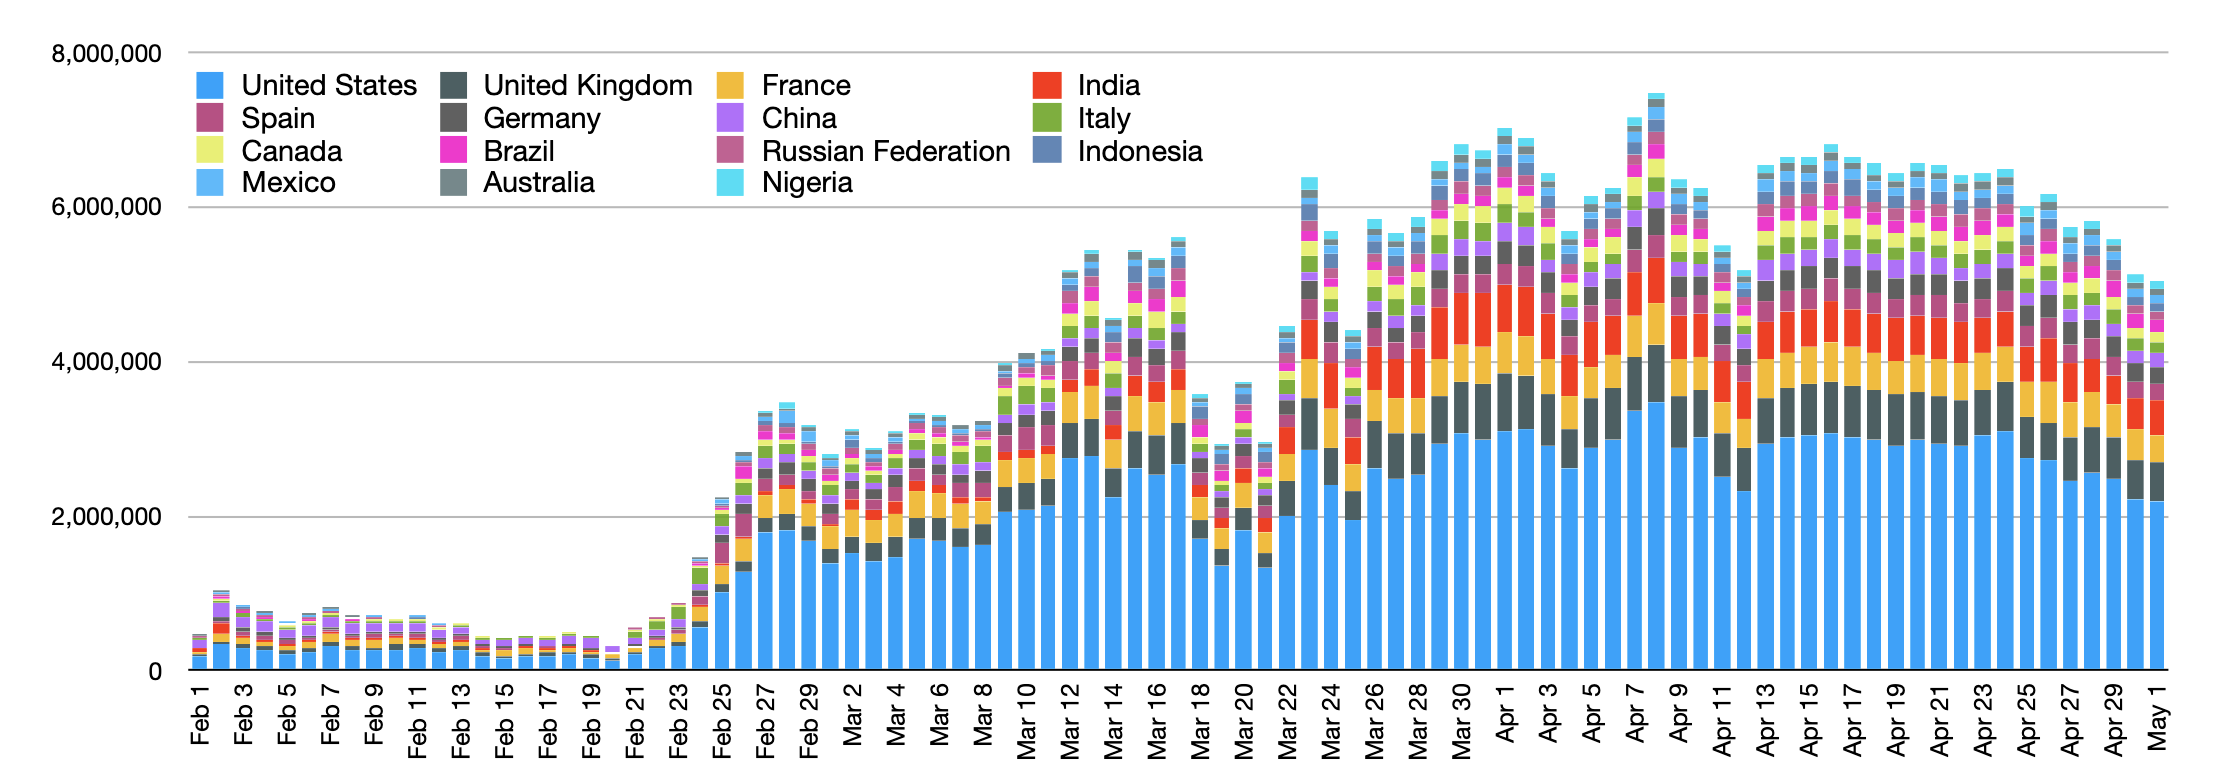
\includegraphics[width=0.8\textwidth]{figs/GeoCov-countrydistribution.png}    
    \centering
    \caption{Daily distribution by country of GeoCoV19 tweets, Feb 1st to May 1st, 2020 \parencite{qaziGeoCoV19DatasetHundreds2020a}}
\end{figure}
%give exact figure instead of 150k here
%https://www.kaggle.com/andradaolteanu/covid-19-sentiment-analysis-social-networks very cool and could be useful!
Of the final dataset, around 150,000 have exact geolocation embedded in the tweet. This is due to the fact that geo-tagging is an explicit option that needs to be set for each tweet, involving activating location data on the mobile app. Another option for geo-tagging is to select a place from a search box; yielding a `place' in the metadata. Both of these types of metadata involve accurate locations, but make up a small proportion of the total geolocated tweets. A third method of geolocating tweets is used to identify most of the locations: when activating a Twitter account the user is strongly encouraged to set their location in their profile. Although it is a free field (generated Place suggestions are included, but are optional), most users set this to their current location; this metadata is included with every tweet. The maintainers of the dataset then employ a toponym extraction approach to elicit the location of the location field. The text of the user location field is first cleaned of non-text characters and symbols. Candidates are then created from the remaining unigrams (single words) and bigrams (pairs of adjacent words), ensuring that two-word place names like `Los Angeles' are included. Groups of three or more words are not considered. Each remaining candidate is filtered against a list of stopwords (see section \ref{textan}), and against the `World Cities Database'\footnote{Available at \texttt{https://www.kaggle.com/max-mind/world-cities-database?select=worldcitiespop.csv}}, an index of 3.1 million worldwide place names, covering 141,989 locations in the US. The remaining candidates are sent as one query to Nominatim, the OpenStreetMap search engine, yielding a best-attempt geolocation: the procedure works best when state and place name is given. Cross-checking the procedure with GPS-geolocated tweets, the dataset shows good coverage and accuracy across US counties, and so makes a panel approach viable. The maintainers of the dataset also presented locations derived from the text of the tweet itself using the same procedure, but we filter these tweets out of the final dataset due to low accuracy. A drawback to this gazeteer approach is that, since users can set their profile location freely, users from other countries or states could masquerade as Americans in particular locations, or the classification process could mis-classify a foreign (particularly English) place as a US location due to sharing a name -- for example, York County, Maine. In order to account for this we remove counties from consideration that have a share of total tweets significantly higher than their population share of the US: Earth, Texas, is the most prominent example of this. Other than misclassification, deliberate setting of the profile location to a US location is possible. This may be a concern for large, well-known cities like Los Angeles and New York, but it is less likely that a given user will set their location to a less well-known American county. Finally, users may move county and not change their location.
\begin{figure}[h!]
    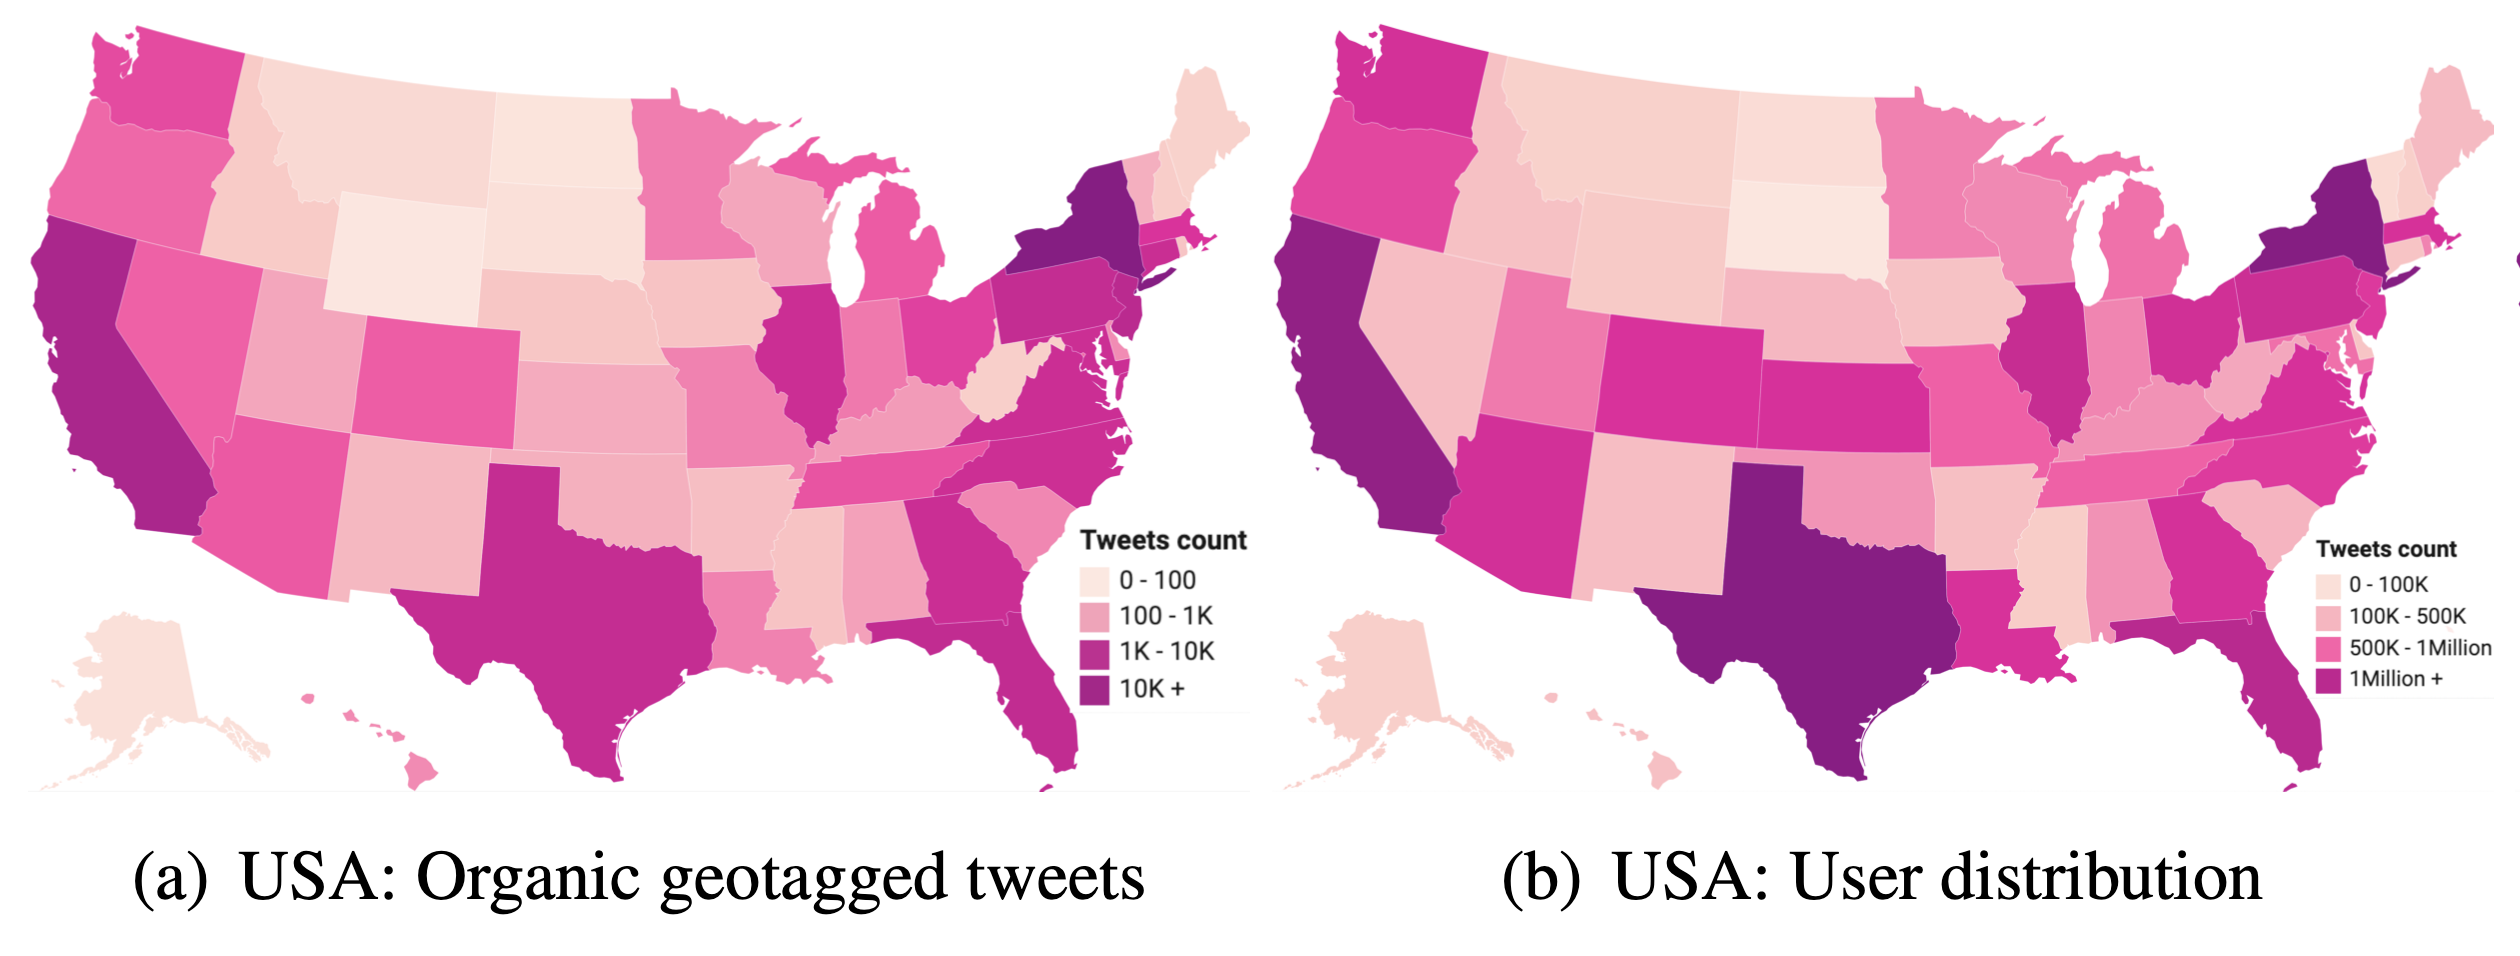
\includegraphics[width=0.8\textwidth]{figs/GeoCov-USdist.png}    
    \centering
    \caption{Geographic distribution of GeoCoV19 tweets and users \parencite{qaziGeoCoV19DatasetHundreds2020a}}
\end{figure}

Twitter's terms of service restrict the large-scale sharing of Tweet datasets; hence public-facing tweet datasets can only be made available `dehydrated', with only the universal identifiers (a long number that maps to the tweet in Twitter's database) given, instead of the tweet text and assorted metadata. In order to use the dataset to analyse tweet content, researchers wishing to use the dataset must apply and be accepted for a Developer account. This gives access to a password called an API key, which is used to query the Twitter API with the identifiers to `rehydrate' and gain access to the full tweet text and metadata. Since the tweets are delivered from the servers at download time, this procedure entails that a proportion of Tweets -- those identified as containing misinformation or those sent by users whose accounts have since been suspended or deleted -- will be unavailable on request from the service when the dataset is `rehydrated'. This presents a selection problem for topics like misinformation, where Twitter enacts a stringent and continuous policy. A prominent concern for my data might be the suspension of Donald Trump's prolific Twitter account; his tweets were a touchstone for right-wing US online conversations. This does not present an issue to my data, however, because tweets interacting with tweets from a deleted account are still available from the API. The deletion rate ultimately encountered during the rehydration process was around 20\%, reflecting the normal removal of machine-generated content.

GeoCoV19 was made available as a dehydrated dataset, containing the tweet identifiers and the inferrred geolocation information. The tweets were rehydrated in December 2020 using Hydrator, an open-source tool made available for academic research by the digital archive organisation Documenting the Now \parencite{summersHydrator2020}. Each tweet is delivered in the Javascript Object Notation (JSON) format: this is a common file standard used to deliver arbitrarily nested data. Each entry contains a `tree', which corresponds to a key-value pair. Each value can itself contain a list of named objects; so, unlike a CSV file, the data is not a `flat' table. An example from the Developer documentation is reproduced below: note the nesting and the metadata delivered with the tweet text. The final dataset contained 63,654,120 tweets and measured approximately 207 GB.

\begin{singlespace}
\begin{lstlisting}[language=json,numbers=none,caption=Example Tweet object JSON file \parencite{twitterinc.DataDictionaryStandard2021}]
{
  "created_at": "Thu Apr 06 15:24:15 +0000 2017",
  "id_str": "850006245121695744",
  "text": "1\/ Today we\u2019re sharing our vision for the future of the Twitter API platform!\nhttps:\/\/t.co\/XweGngmxlP",
  "user": {
    "id": 2244994945,
    "name": "Twitter Dev",
    "screen_name": "TwitterDev",
    "location": "Internet",
    "url": "https:\/\/dev.twitter.com\/",
    "description": "Your official source for Twitter Platform news, updates & events. Need technical help? Visit https:\/\/twittercommunity.com\/ \u2328\ufe0f #TapIntoTwitter"
  },
  "place": {   
  },
  "entities": {
    "hashtags": [      
    ],
    "urls": [
      {
        "url": "https:\/\/t.co\/XweGngmxlP",
        "unwound": {
          "url": "https:\/\/cards.twitter.com\/cards\/18ce53wgo4h\/3xo1c",
          "title": "Building the Future of the Twitter API Platform"
        }
      }
    ],
    "user_mentions": [     
    ]
  }
}
\end{lstlisting}
\end{singlespace}
After the dataset downloaded, a Python script was used to parse and un-nest the JSON files, select the relevant variables, and write them to a CSV file. This file was then joined by matching the UIDs in the CSV with the geolocation dataset in GeoCoV19, yielding a large CSV-format dataset containing the tweet text and metadata from Twitter, and inferred geolocation information from GeoCoV19. Language processing was then performed on the tweet text, as is detailed in section \ref{approach}.

\subsection{SafeGraph: Geolocated smartphone data for measuring social distancing}
A second central dataset is provided by SafeGraph, a company which usually collects data on commercial footfall, but made their dataset available for academic research in light of the pandemic. The social distancing dataset was downloaded in January 2020 using the provided API key. The data was parsed and loaded into R using the SafeGraphR package \parencite{huntington-kleinSafeGraphR2020}. The SafeGraph dataset consists of over 45 million anonymised smartphone GPS pings located to an accuracy of a ~150m square location \parencite{safegraphinc.SocialDistancingMetrics2020}. Since the data was collected in 2019 and 2020, year-on-year change can also be presented. The data is presented at district level, but for the purposes of the analysis I aggregated this to a county-level daily metric. For each device on each day, the most common night-time location is determined from the previous 6 weeks. This home location is used to determine the number of devices in a county which leave their home, the length and time of day they leave and return, the district they travel to, and the points of interest they visit. Although this is a sensible method of determining a device's `home', it may be a source of measurement error if an individual works a night shift, does not bring their smartphone with them when they leave the house, or sleeps regularly at a partner's house \parencite{chiouSocialDistancingInternet}. However, I believe that the long lead time of 6 weeks' determination, the large sample size, and the rarity of this occurence mitigate the size of the potential measurement error. There is also a chance for selection bias: the data does not represent those Americans who do not own a GPS-enabled smartphone, and does not represent those who refuse to allow GPS tracking on their smartphones. We assume, with evidence, that these omitted populations are mean-zero with respect to social distancing mobility behaviour: 81\% of US adults own a smartphone and 96\% own a cellphone \parencite{pewresearchcenterDemographicsMobileDevice2019}, and \parencite{atheyDigitalPrivacyParadox2017} indicates that the decision to share personal information has a large random element \parencite{chiouSocialDistancingInternet}. SafeGraph also address the issue of sampling bias\footnote{\tt{https://colab.research.google.com/drive/1u15afRytJMsizySFqA2EPlXSh3KTmNTQ\#sandboxMode=true}} by comparing, for each census block, the observed proportion of all devices to that census block's proportion of total US population\footnote{That is, if New York County has 3.14\% of the US population, they would expect to find 3.14\% of their total observed devices in New York County}. They assess this sampling bias at the county and demographic level and do not find a significant in observed proportion to that indicated by the census data. From this rich data, I derive two primary variables: the median minutes spent at home during 8am-6pm and the proportion of measured devices that stayed at home all day.  It should be noted that the differential anonymisation means that the exact sum of devices is inaccurate; although there is a possibility to bias the proportions I calculate, this only arises in areas which are sparsely populated. These areas usually do not yield enough geo-located tweets to be included in the final analysis, so the problem is largely circumvented.

\subsection{Other datasets}
\subsubsection{Oxford COVID-19 Government Response Index}
An ongoing feature of the US response to COVID-19 is the differential policies enacted in each state. These policies had varying effects on the extent of social distancing practised in the state and sub-state areas. In order to account for this variation, it is necessary to report the nature and strength of the policy in place in each county at each time point. \textcite{petherickVariationGovernmentResponses2020} provide the \textit{de facto} standard index for tracking government responses. This dataset, originating from the Blavatnik School of Government at Oxford University, reports 19 indicators of government response in containment/control, economic support, and health categories. The containment/control variables are of most interest; these include indicators for school/workplace closures, public transport closures, stay at home requirements, internal/international movement restrictions, restrictions on gathering size, and public event cancellation. These are coded on an ordinal scale (usually 0 to 2, but sometimes 0 to 4), measuring the severity or intensity of the policy. These indicator variables are then aggregated into a `policy stringency' index, a numeric measure of the general severity of restrictions on movement in a governmental area. This index is created by taking the ordinal values of each indicator, rescaling each by the maximum value of the scale, to create a score between 0 and 100. Although this approach inevitably masks substantial subtleties in the context of each policy, they crucially provide a comparable index. The dataset is available at the state level for the US, meaning that it does not cover county-level differences in policy. However, this does not present a problem for the analysis; practically all non-federal COVID containment policies were enacted by blanket state-level orders.

\subsubsection{American Community Survey and Census}
Demographics also have a significant bearing on social distancing behaviour; an area with more elderly people will display less movement than a younger district, due both to baseline movement patterns and differing shielding behaviours during the pandemic. In the main specifcation, we account for this with county fixed effects; but this data is also useful for exploring patterns of sentiment and social distancing among broader demographics. Therefore, I include data from the American Community Survey (ACS) and the 2011 US Census. This includes variables like population density, income, and age distribution. I match the Public Use Microdata Sample of the ACS to the county level, the smallest level available. 
\subsection{Descriptive statistics}

\section{Methods}
\subsection{Text analysis for Twitter data: approach taken}\label{approach}
\subsubsection{NRC Emotion Lexicon}
Sentiment analysis is the task of inferring the author's opinion of a subject from the text they write about that subject. Due to major commercial incentives for accurate sentiment inference from internet companies, this area has seen major advancement over the last 15 years. The NRC Emotion Lexicon is a widely-used tool in this field; the project aims to answer the question ``Is the author happy with, angry at, or fearful of the target?'' \parencite{mohammadCrowdsourcingWordEmotion2013}. In the broadest sense, this attitude towards the subject of the text is called the text's \textit{polarity}, which is either positive, neutral, or negative. As such, most indexes of polarity are reported on a scale of \([0,1]\). 
\subsubsection{\texttt{szuyhet} R package and workflow}
\subsubsection{The VADER package}

\subsection{Empirical model}
Given this county-level measure of tweet sentiment, we now incorporate it into an empirical model of social distancing.
\subsubsection{Inference with Panel Fixed Effects}
\subsubsection{Specifications and hypotheses}

\section{Results}%1000 words

\subsection{Robustness checks}

\section{Discussion and conclusion} %1000 words


\printbibliography

\end{document}